\PassOptionsToPackage{unicode=true}{hyperref} % options for packages loaded elsewhere
\PassOptionsToPackage{hyphens}{url}
%
\documentclass[]{article}
\usepackage{lmodern}
\usepackage{amssymb,amsmath}
\usepackage{ifxetex,ifluatex}
\usepackage{fixltx2e} % provides \textsubscript
\ifnum 0\ifxetex 1\fi\ifluatex 1\fi=0 % if pdftex
  \usepackage[T1]{fontenc}
  \usepackage[utf8]{inputenc}
  \usepackage{textcomp} % provides euro and other symbols
\else % if luatex or xelatex
  \usepackage{unicode-math}
  \defaultfontfeatures{Ligatures=TeX,Scale=MatchLowercase}
\fi
% use upquote if available, for straight quotes in verbatim environments
\IfFileExists{upquote.sty}{\usepackage{upquote}}{}
% use microtype if available
\IfFileExists{microtype.sty}{%
\usepackage[]{microtype}
\UseMicrotypeSet[protrusion]{basicmath} % disable protrusion for tt fonts
}{}
\usepackage{hyperref}
\hypersetup{
            pdftitle={The 2019-20 NBA Season: What Could Have Been},
            pdfauthor={Ryan Kohanski; Rithvik Saravanan; Howard Yong},
            pdfborder={0 0 0},
            breaklinks=true}
\urlstyle{same}  % don't use monospace font for urls
\usepackage[margin=1in]{geometry}
\usepackage{longtable,booktabs}
% Fix footnotes in tables (requires footnote package)
\IfFileExists{footnote.sty}{\usepackage{footnote}\makesavenoteenv{longtable}}{}
\usepackage{graphicx,grffile}
\makeatletter
\def\maxwidth{\ifdim\Gin@nat@width>\linewidth\linewidth\else\Gin@nat@width\fi}
\def\maxheight{\ifdim\Gin@nat@height>\textheight\textheight\else\Gin@nat@height\fi}
\makeatother
% Scale images if necessary, so that they will not overflow the page
% margins by default, and it is still possible to overwrite the defaults
% using explicit options in \includegraphics[width, height, ...]{}
\setkeys{Gin}{width=\maxwidth,height=\maxheight,keepaspectratio}
\setlength{\emergencystretch}{3em}  % prevent overfull lines
\providecommand{\tightlist}{%
  \setlength{\itemsep}{0pt}\setlength{\parskip}{0pt}}
\setcounter{secnumdepth}{0}
% Redefines (sub)paragraphs to behave more like sections
\ifx\paragraph\undefined\else
\let\oldparagraph\paragraph
\renewcommand{\paragraph}[1]{\oldparagraph{#1}\mbox{}}
\fi
\ifx\subparagraph\undefined\else
\let\oldsubparagraph\subparagraph
\renewcommand{\subparagraph}[1]{\oldsubparagraph{#1}\mbox{}}
\fi

% set default figure placement to htbp
\makeatletter
\def\fps@figure{htbp}
\makeatother

\usepackage{float}

\title{The 2019-20 NBA Season: What Could Have Been}
\author{Ryan Kohanski \and Rithvik Saravanan \and Howard Yong}
\date{May 11, 2020}

\begin{document}
\maketitle

\hypertarget{abstract}{%
\section{Abstract}\label{abstract}}

The COVID-19 pandemic has affected our society in various ways and has
changed numerous events on schedule for 2020. One such event that we
were looking forward to was the end of the 2019-20 NBA season as well as
the 2020 NBA Playoffs. Since a large portion of the 2019-20 NBA regular
season games have already been played, we utilized the data collected
from these games to run regression prediction models and calculate Elo
ratings for each team in order to predict the standings for 2019-20 as
well as the matchups and results of the Playoffs and the NBA season
awards. Running our analysis by predicting the 7-game playoff series
matchups, we predicted that the Western Conference Finals matchup will
be between the \#1 seed Los Angeles Lakers and the \#2 seed Los Angeles
Clippers and the Eastern Conference Finals matchup will be between the
\#1 seed Milwaukee Bucks and the \#2 seed Toronto Raptors.
\textbf{{[}NEED TO FIX THE MATCHUPS BASED ON BRACKET{]}} We found that
running these simulations predicts the NBA Finals matchup between the
Los Angeles Lakers and the Milwaukee Bucks with the Los Angeles Lakers
ultimately claiming the Larry O'Brien NBA Championship Trophy.
Additionally, we used several types of regression models to best predict
end-of-season statistics for every player. We ultimately used a logistic
regression model to predict the end-of-season statistics and leaders for
each of the major categories and found that our predictions indicate
that Giannis Antetokounmpo will claim both the NBA Most Valuable Player
(MVP) award as well as the Defensive Player of the Year (DPOY) award.
According to our prediction model, this will mark only the third time in
NBA history that a player will win MVP and DPOY in the same season with
the previous two players being basketball legends Michael Jordan and
Hakeem Olajuwon.

\hypertarget{introduction}{%
\section{Introduction}\label{introduction}}

Due to the widespread impact of the COVID-19 pandemic throughout the
world, almost every company, organization, and public event has canceled
or suspended any activities that involve interpersonal contact for the
forseeable future. Many of these activities are moving to a virtual
format if possible, but several others have been forced to shut down.

As avid sports fans, the absence of the major sporting events during
this time has hit us and many others around the world especially hard
{[}1{]}. Some of the events that we particularly were looking forward to
include the NBA, NCAA March Madness tournament, MLB, and the 2020 Summer
Olympics.

In our curiosity, we decided to utilize this opportunity to exercise our
data science and modeling skills in order to predict what could have
been. Specifically, we focused on the NBA and the NBA Playoffs. Since
the 2019-20 NBA season was suspended approximately one month prior to
the end of the regular season (and the beginning of the Playoffs), we
used the 2019-20 season data accumulated from the games played before
the suspension to predict how the season and the Playoffs would have
ended had everything gone according to schedule.

In this analysis, we will examine data from the 2019-20 NBA season as
well as some data from previous NBA seasons in order to draw some
meaningful conclusions about the remainder of the 2019-20 NBA season
including the final season standings, playoff matchups, championship
winner, and season award winners.

\hypertarget{methods}{%
\section{Methods}\label{methods}}

\hypertarget{predicting-the-2019-20-nba-season-standings}{%
\subsection{Predicting the 2019-20 NBA Season
Standings}\label{predicting-the-2019-20-nba-season-standings}}

Since we missed one of the most exciting times of the year (the NBA
Playoffs \& Finals), we made some predictions on how the rest of the
season might have played out using a popular methodology referred to as
the Elo ratings system {[}2{]}. This tool, created by Hungarian-American
physics professor Arpad Elo, was orginally designed to rate chess
players, but is now used for all sorts of competitions ranging anywhere
from sports to video games. This is a methodology that FiveThirtyEight
and many other popular sports analysts take advantage of due to its
simplicity and effectiveness {[}3{]}.

These ratings depend only on the final score of each game as well as
where it was played (home-court advantage). In other words, this system
is built on a Win/Loss basis. We will be analyzing the 2018-19 NBA
Season in its entirety to validate its performance, then we will apply
it to the 2019-20 regular season in order to predict the matchups for
the Playoffs and the Finals and ultimately the NBA Champions. For this
project, we retrieved several types of data sources including
game-by-game scores and schedules for several seasons from
Basketball-Reference.com {[}4{]}.

\hypertarget{how-does-elo-work}{%
\subsubsection{How does Elo work?}\label{how-does-elo-work}}

The long-run average for an Elo score in the NBA sits around 1500. An
Elo of 1500 means that the teams performance would be normally
distrubuted around an average of 1500 with the chance of performing
better or worse. For more detail, Figure \ref{fig:elo_chart} (Appendix)
shows what an Elo rating tells us about a team and how it can convey the
teams overall season record. A higher Elo rating indicates that the team
has a high win-loss ratio and is more likely to play deeper into the
season.

The formula for Elo below shows how the probability of one team beating
another is calculated using the ratings. When Player \(A\) competes in a
match against Player \(B\), Player \(A\) has an expected outcome
(probability or score) for Team \(A\) (\(E[A]\)) where \(R_A\) is the
rating for Team \(A\) and \(R_B\) is the rating for Team \(B\). The
expected outcome for Team \(A\) (\(E[A]\)) can be calculated by the
formula below:

\[
E[A] = \frac{1}{1 + 10^{\frac{(R_B-R_A)}{400}}}
\]

The same calculation (\(E[B]\)) has to be done for Player \(B\), but
with \(R_A\) (current rating \(A\)) and \(R_B\) (current rating \(B\))
swapped so that \(E[A] + E[B] = 1\). Once the match is played and
\(S_A\) (actual outcome or score for Team \(A\)) and \(S_B\) (actual
outcome or score for Team \(B\)) are determined, \(R^{\prime}_A\) (the
new rating for \(A\)) and \(R^{\prime}_B\) (the new rating for \(A\))
are calculated with the formula below:

\[
R^{\prime}_A=R_A+K(S_A-E[A])
\]

The \(S\) value in our case would either be 1 for a win, or 0 for a
loss. This is because there are no ties in the NBA.

In this equation, \(K\) is an optimization constant that usually takes
different values according the sport and the amount of games available.
In other words, this value is the maximum amount by which a score can
change in one match. If \(K\) is set too high, the ratings will jump
around too much; if \(K\) is set too low, Elo will take too long to
recognize important changes in team quality. Determining the right value
of K is an entirely different and more complicated topic, so for this
experiment we will be using \(K=20\), the optimal \(K\) for the NBA
determined by FiveThirtyEight {[}3{]}. This is higher than most other
sports and can likely be attributed to the fact that the NBA plays more
games (81 games per team) and is subject to relatively little
randomness.

Home-court advantage is set as equivalent to 100 Elo rating points. One
hundred Elo points is equivalent to about 3.5 NBA points, so it can also
be interpreted as the home team being favored by 3 to 4 points if the
teams were otherwise evenly matched (obviously this value fluctuates
from season to season). Since every team plays about half of their games
at home and the other half away, a change in the home-court advantage
value does not produce a significant difference in the ratings, but is
still an important factor to consider.

Elo strikes a nice balance between ratings systems that account for
margin of victory and those that do not. While teams always gain Elo
points after wins and lose Elo points after losses, they also gain or
lose more with larger margins of victory.

This works by assigning a multiplier to each game based on the final
score and dividing it by a team's projected margin of victory
conditional upon having won the game. For instance, the Golden State
Warriors' 4-point margin over the Houston Rockets in Game 1 of the
2018-19 Western Conference finals was lower than Elo would expect for a
Warriors win. So the Warriors gain Elo points, but not as many as if
they'd won by a larger margin. The formula accounts for diminishing
returns; going from a 5-point win to a 10-point win matters more than
going from a 25-point win to a 30-point win. For the exact formula, see
the footnotes.

Instead of resetting each team's rating when a new season begins, Elo
carries over a portion of a team's rating from one season to the next.
This is to account for any momentum that a team may build from
season-to-season (i.e.~sports dynasties). In NBA ratings, three-quarters
of the previous score are kept. The high fraction reflects the fact that
NBA teams are more consistent from year to year. For example, the Miami
Heat ended the 2012-13 NBA season with an Elo rating of 1754. The team's
Elo rating for the start of the 2013-14 season is calculated as follows:

\[
(0.75 * 1754) + (0.25 * 1500) = 1692
\]

Since this is a consistent method, we will also initialize the Elo
scores for the 2019-20 NBA Season using the Elo scores from the 2018-19
season.

After incorporating a constant for home court advantage, our formula is
as follows with \(A=100\) points (the value we previously determined
represents a home-court advantage):

\[
P(\mbox{Home team wins}) = \frac{1}{1 + 10^{-\frac{(H-R+A)}{400}}}
\]

\begin{figure}[H]

{\centering 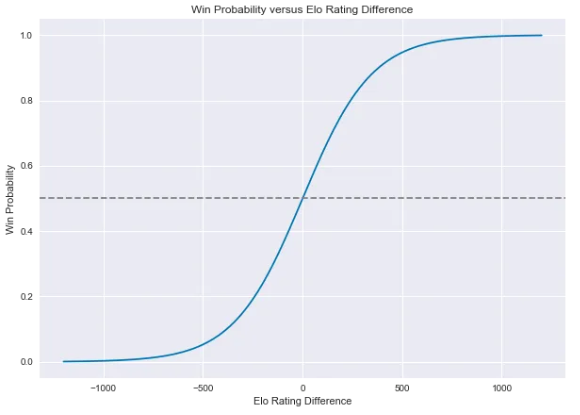
\includegraphics[width=.49\linewidth]{./logistic} 

}

\caption{\label{fig:logit}Logistic Function of Win Probability by Elo Rating Difference}\label{fig:elo_logit}
\end{figure}

In Figure \ref{fig:logit}, we see an example of a logistic function for
win probability by Elo rating difference.

\hypertarget{calculating-elo-ratings}{%
\subsubsection{Calculating Elo Ratings}\label{calculating-elo-ratings}}

For our project scope, we decided to model our Elo rating system purely
off of home court advantage, wins, losses, and point margin
differentials. Of course, in the NBA, there is a wide array of different
factors to consider, including roster changes, injuries, winning
streaks, etc. These are all features that limit the capabilities of our
model, but serve as potential targets of investigation for the future.
As we mentioned before, one principal task of our project was to explore
outcomes of the 2019-20 NBA season if they were to continue. In order to
do so, we first needed to develop Elo ratings for each team at their
current state of the 2019-20 season. Online resources report that the
NBA has historically shown an average Elo rating of 1505, as the league
is continually experiencing expansions and contractions that influence
the center of the distribution of team ratings. We followed this
statistic in our Elo rating calculations. When simulating Elo rating
calculations for each team throughout multiple seasons, we preemptively
decided to carry over 75\% of each team's Elo rating from the previous
season, with the other 25\% weight carried by the league average of
1505. This proportion was determined through historical league analyses
of the NBA.

For the scope of our analysis, we decided to begin our analysis in the
2016-17 NBA season. We chose to start our calculations from this season
because the season data was readily available and provided enough years
to build a more-updated status of each team's current standing in the
league. We started by scraping online sources for box score statistics
for each team. Our source for basketball statistics for Elo rating
calculations came from basketball-reference. Once we scraped and
processed the data, we exported them into indepdent .csv files for each
season. Below is an example of data from the 2019-20 NBA season we
collected.

\begin{verbatim}
##        game_id  date_game game_start_time      visitor_team_name visitor_pts
## 1 201910220TOR 2019-10-22           8:00p   New Orleans Pelicans         122
## 2 201910220LAC 2019-10-22          10:30p     Los Angeles Lakers         102
## 3 201910230CHO 2019-10-23           7:00p          Chicago Bulls         125
## 4 201910230IND 2019-10-23           7:00p        Detroit Pistons         119
## 5 201910230ORL 2019-10-23           7:00p    Cleveland Cavaliers          85
## 6 201910230BRK 2019-10-23           7:30p Minnesota Timberwolves         127
##         home_team_name home_pts overtimes attendance game_remarks
## 1      Toronto Raptors      130        OT      20787             
## 2 Los Angeles Clippers      112                19068             
## 3    Charlotte Hornets      126                15424             
## 4       Indiana Pacers      110                17923             
## 5        Orlando Magic       94                18846             
## 6        Brooklyn Nets      126        OT      17732             
##   home_team_wins
## 1              1
## 2              1
## 3              1
## 4              0
## 5              1
## 6              0
\end{verbatim}

Once we had all the data collected for the season, we calculated the Elo
ratings by the same methods previously mentioned. We iterated through
the season by each matchup, calculating and updating the Elo ratings for
the teams playing simultaneously, and applied this to every season until
2019-20.

Below is an example of what the teams Elo ratings looked like at the end
of the 2016-2017 season, the year that Kevin Durant made the
controversial move to the Golden State Warriors and took them on a
championship run.

\begin{verbatim}
##                      team       elo
## 1   Golden State Warriors 1834.8023
## 2       San Antonio Spurs 1641.0866
## 3     Cleveland Cavaliers 1637.0718
## 4         Houston Rockets 1613.1483
## 5               Utah Jazz 1595.1288
## 6    Los Angeles Clippers 1590.3924
## 7          Boston Celtics 1589.2328
## 8      Washington Wizards 1578.5608
## 9         Toronto Raptors 1557.6831
## 10             Miami Heat 1551.7687
## 11  Oklahoma City Thunder 1536.7487
## 12 Portland Trail Blazers 1530.7001
## 13         Denver Nuggets 1526.9812
## 14        Milwaukee Bucks 1511.4234
## 15          Chicago Bulls 1496.4171
## 16      Memphis Grizzlies 1488.3390
## 17          Atlanta Hawks 1486.4438
## 18         Indiana Pacers 1475.5359
## 19   New Orleans Pelicans 1468.9413
## 20       Dallas Mavericks 1437.5093
## 21      Charlotte Hornets 1432.4283
## 22        Detroit Pistons 1432.1112
## 23       Sacramento Kings 1422.6389
## 24 Minnesota Timberwolves 1420.9144
## 25        New York Knicks 1380.9276
## 26     Los Angeles Lakers 1372.8674
## 27          Orlando Magic 1368.1960
## 28     Philadelphia 76ers 1360.4503
## 29          Brooklyn Nets 1331.6848
## 30           Phoenix Suns 1329.8653
\end{verbatim}

After our calculations, we were obtain the Elo ratings of the NBA teams
at the beginning of the 2019-20 season. We tracked their progress
throughout this year's season and plotted them in the figure below. The
plot is facetted by conferences, which determines how many times a team
plays other teams, as well as who they may contend against in their
playoff runs. The current Elo ratings of each team in the league can be
found below.

\hypertarget{simulations-and-predictions}{%
\subsubsection{Simulations and
Predictions}\label{simulations-and-predictions}}

After calculating the Elo ratings for each NBA team up until the last
game they played (before the season was suspended), we used these
ratings to then perform simulations matching up teams based on the rest
of the season schedule as well as the post-season tournaments based on
the top seeded teams from the regular season.

\includegraphics{report_files/figure-latex/unnamed-chunk-6-1.pdf}

\hypertarget{the-remaining-2019-2020-regular-season}{%
\subparagraph{The Remaining 2019-2020 Regular
Season}\label{the-remaining-2019-2020-regular-season}}

Since the 2019-2020 season was cancelled before the end of the regular
season, there were still more games to be played. Fortunately, we were
able to scrape the remaining schedule that includes all the games that
were supposed to happen for the rest of the regular season. The schedule
looked something like so:

\begin{verbatim}
##   id         visitor_team              home_team       time     tv       date
## 1  0            Utah Jazz  Oklahoma City Thunder  8:00 p.m. NBA LP 03-11-2020
## 2  1 New Orleans Pelicans       Sacramento Kings 10:00 p.m.   ESPN 03-11-2020
## 3  2        Chicago Bulls          Orlando Magic  7:00 p.m. NBA LP 03-12-2020
## 4  3       Boston Celtics        Milwaukee Bucks  8:00 p.m.    TNT 03-12-2020
## 5  4    Memphis Grizzlies Portland Trail Blazers 10:00 p.m. NBA LP 03-12-2020
## 6  5        Brooklyn Nets  Golden State Warriors 10:30 p.m. NBA LP 03-12-2020
\end{verbatim}

The regular season would have lasted all the way through April. Since we
have all the matchups, we can run these teams through a simulation to
compete based on probability using their elo ratings. This involved
looping through the dataset, pulling each teams elo rating to calculate
their probability of winning or losing, and then pulling a random sample
as the winner. After the winner is found, the elo ratings are then
updated to reflect this outcome.

To get an understanding of these results, we added the winners of each
match to the dataframe next to each game.

\begin{verbatim}
##   id         visitor_team              home_team       time     tv       date
## 1  0            Utah Jazz  Oklahoma City Thunder  8:00 p.m. NBA LP 03-11-2020
## 2  1 New Orleans Pelicans       Sacramento Kings 10:00 p.m.   ESPN 03-11-2020
## 3  2        Chicago Bulls          Orlando Magic  7:00 p.m. NBA LP 03-12-2020
## 4  3       Boston Celtics        Milwaukee Bucks  8:00 p.m.    TNT 03-12-2020
## 5  4    Memphis Grizzlies Portland Trail Blazers 10:00 p.m. NBA LP 03-12-2020
## 6  5        Brooklyn Nets  Golden State Warriors 10:30 p.m. NBA LP 03-12-2020
##                 winners
## 1 Oklahoma City Thunder
## 2  New Orleans Pelicans
## 3         Orlando Magic
## 4       Milwaukee Bucks
## 5     Memphis Grizzlies
## 6 Golden State Warriors
\end{verbatim}

This finalized the regular season, resulting in the updated elo scores
going into the playoffs.

\begin{verbatim}
##     X                   team       elo
## 1  23     Los Angeles Lakers 1848.7423
## 2  17         Boston Celtics 1783.4930
## 3  24        Milwaukee Bucks 1761.1672
## 4  15        Houston Rockets 1706.1507
## 5  20  Oklahoma City Thunder 1686.4824
## 6   2   Los Angeles Clippers 1685.8538
## 7   7             Miami Heat 1679.5070
## 8   1        Toronto Raptors 1678.4602
## 9  21         Denver Nuggets 1678.2816
## 10 18      Memphis Grizzlies 1636.2577
## 11 11              Utah Jazz 1629.9049
## 12  4         Indiana Pacers 1624.6260
## 13  5          Orlando Magic 1607.1807
## 14  8     Philadelphia 76ers 1591.7260
## 15  6          Brooklyn Nets 1582.9383
## 16 19   New Orleans Pelicans 1559.2897
## 17 13 Portland Trail Blazers 1555.0463
## 18 29 Minnesota Timberwolves 1547.0046
## 19  9       Dallas Mavericks 1537.8738
## 20 10      San Antonio Spurs 1527.0983
## 21 22       Sacramento Kings 1522.6547
## 22 30     Washington Wizards 1511.4908
## 23 25          Atlanta Hawks 1493.7892
## 24 16  Golden State Warriors 1491.3453
## 25  3      Charlotte Hornets 1485.9334
## 26 12           Phoenix Suns 1483.2909
## 27 26        New York Knicks 1387.9954
## 28 27          Chicago Bulls 1375.6587
## 29 14        Detroit Pistons 1352.8493
## 30 28    Cleveland Cavaliers 1326.2108
\end{verbatim}

\hypertarget{the-2019-2020-nba-playoffs}{%
\subparagraph{The 2019-2020 NBA
Playoffs}\label{the-2019-2020-nba-playoffs}}

For the NBA playoffs, the top 8 teams in terms of win/loss record from
each conference (Eastern Conference \& Western Conference) advance to
the playoffs. The teams are then seeded (ranked) based on these win/loss
records, and matched accordingly for the playoffs. This means the \#1
seed plays the \#8 seed, the \#2 seed plays the \#7 seed, the the \#3
seed plays the \#6 seed, and the \#4 seed plays the \#5 seed, in each
conference. Since the seedings are based on win/loss, we found it
appropriate to seed the teams based on elo ratings (which is an outcome
of win/loss). This also helps to avoid the complicated process should
two teams have the same win loss record (there is a significantly lower
probability two teams in this case have the exact same elo score). This
is how the first round playoff matchups turned out:

\begin{verbatim}
##                   team1                team2
## 1    Los Angeles Lakers New Orleans Pelicans
## 2       Houston Rockets    Memphis Grizzlies
## 3  Los Angeles Clippers       Denver Nuggets
## 4 Oklahoma City Thunder            Utah Jazz
## 5       Milwaukee Bucks        Brooklyn Nets
## 6        Boston Celtics   Philadelphia 76ers
## 7       Toronto Raptors        Orlando Magic
## 8            Miami Heat       Indiana Pacers
\end{verbatim}

The same process for the regular season was applied to these matchups
with a couple of tweaks. For starters, this simulation was a best-of-7
tournament (as are all playoffs and finals matches). This means we had
to simulate the games until a team reached 4 wins. The teams who won the
right to advance to the second round are as follows:

\begin{verbatim}
## [1] "Los Angeles Lakers"    "Memphis Grizzlies"     "Denver Nuggets"       
## [4] "Oklahoma City Thunder" "Milwaukee Bucks"       "Boston Celtics"       
## [7] "Toronto Raptors"       "Miami Heat"
\end{verbatim}

The second round is the same process as the first round, except this
time, the top 4 teams of each conference advance, meaning that the other
4 finish their season early. The second round is also known as the
conference semifinals, that is, the winners of these games advance to
their respective conference finals to compete for the conference title.
The second round matchups are shown below:

\begin{verbatim}
##                team1                 team2
## 1 Los Angeles Lakers     Memphis Grizzlies
## 2     Denver Nuggets Oklahoma City Thunder
## 3    Milwaukee Bucks        Boston Celtics
## 4    Toronto Raptors            Miami Heat
\end{verbatim}

with the winners being:

\begin{verbatim}
## [1] "Los Angeles Lakers" "Denver Nuggets"     "Boston Celtics"    
## [4] "Miami Heat"
\end{verbatim}

The last round of the playoffs is the third round, also referred to as
the conference finals. The top two teams from both the western and
eastern conference compete for the top spot in their respective
conference. The winners that advanced from the second round are:

\texttt{\{r.\ echo=FALSE\}\ conference}

Again, these teams were put through a best-of-7 simulation, in whcih the
following winners emerged:

\begin{verbatim}
## [1] "Los Angeles Lakers" "Boston Celtics"
\end{verbatim}

Finally, the NBA Finals. This is where the top winning teams from each
conference (also the conference champions), compete head-to-head for the
season. For our simu;ation, this turned out to be:

\begin{verbatim}
##                team1          team2
## 1 Los Angeles Lakers Boston Celtics
\end{verbatim}

with the 2019-2020 NBA Champions being\ldots{} \emph{drum roll}\ldots{}

\begin{verbatim}
## [1] "Los Angeles Lakers"
\end{verbatim}

\hypertarget{end-of-season-elo-ratings}{%
\subparagraph{End of Season Elo
Ratings}\label{end-of-season-elo-ratings}}

After all is settled, the final elo ratings after the 2019-2020 NBA
season turned out to be:

\begin{verbatim}
##     X                   team       elo
## 1   1        Toronto Raptors 1678.4602
## 2   2   Los Angeles Clippers 1685.8538
## 3   3      Charlotte Hornets 1485.9334
## 4   4         Indiana Pacers 1624.6260
## 5   5          Orlando Magic 1607.1807
## 6   6          Brooklyn Nets 1582.9383
## 7   7             Miami Heat 1679.5070
## 8   8     Philadelphia 76ers 1591.7260
## 9   9       Dallas Mavericks 1537.8738
## 10 10      San Antonio Spurs 1527.0983
## 11 11              Utah Jazz 1629.9049
## 12 12           Phoenix Suns 1483.2909
## 13 13 Portland Trail Blazers 1555.0463
## 14 14        Detroit Pistons 1352.8493
## 15 15        Houston Rockets 1706.1507
## 16 16  Golden State Warriors 1491.3453
## 17 17         Boston Celtics 1783.4930
## 18 18      Memphis Grizzlies 1636.2577
## 19 19   New Orleans Pelicans 1559.2897
## 20 20  Oklahoma City Thunder 1686.4824
## 21 21         Denver Nuggets 1678.2816
## 22 22       Sacramento Kings 1522.6547
## 23 23     Los Angeles Lakers 1848.7423
## 24 24        Milwaukee Bucks 1761.1672
## 25 25          Atlanta Hawks 1493.7892
## 26 26        New York Knicks 1387.9954
## 27 27          Chicago Bulls 1375.6587
## 28 28    Cleveland Cavaliers 1326.2108
## 29 29 Minnesota Timberwolves 1547.0046
## 30 30     Washington Wizards 1511.4908
\end{verbatim}

You can find visuals of how these elo ratings changed throughout this
process in the results section of this report.

\hypertarget{predicting-the-2019-20-nba-season-award-winners}{%
\subsection{Predicting the 2019-20 NBA Season Award
Winners}\label{predicting-the-2019-20-nba-season-award-winners}}

Another interesting part of any NBA season is the awards given to the
players and teams based on their regular season performances. Some key
awards that catch headlines every year include Most Valuable Player
(MVP) and Defensive Player of the Year (DPOY). In addition to predicting
the end-of-season standings, we decided that any analysis of the
remainder of the 2019-20 NBA season would be incomplete unless it
discussed award winners in the major categories. As avid basketball
fans, this idea resonated with us so we decided to scientifically
predict who would ultimately win the MVP and DPOY awards.

In order to predict award winners at the end of the season, we needed to
predict the leaders of some of the crucial statistical categories at the
end of the season. To predict these players, we analyzed some
significant statistics and identified the optimal regression model to
predict these statistics. Some of the statistics we utilized in building
this model include true shooting percentage (TS\%), total rebound
percentage (TRB\%), assist percentage (AST\%), and block percentage
(BLK\%) among 22 total recorded categories. For additional information
on the exact statistics that were used in these predictions, refer to
Table 3 (Appendix).

Accordingly, we examined different types of regression models in order
to identify which type of model best predicted some of the major
statistics. These include win shares (WS), value over replacement player
(VORP), player efficiency rating (PER), usage percentage (USG\%),
offensive box plus/minus (OBPM), and defensive box plus/minus (DBPM).
For more detailed explanations of the significance of each of these
statistics, refer to Table 3 (Appendix).

To identify the best prediction model, we first predicted WS from the
current 2019-20 season statistics using 4 different regression models:
linear, lasso, ridge, and logistic. We measured the performance of every
model with the actual WS values for each player using RMSE (root mean
squared error) to determine which had the least error where smaller RMSE
values indicated higher accuracy. In order to reduce Monte Carlo
variability, we used 200 repeated random samples of the data for each
model to find the true RMSE values.

We then used this to predict the MVP and DPOY by looking at the leaders
at the end of the season in WS, VORP, PER, USG\%, OBPM, and DBPM because
these categories carried significant weighting in determing the
respective awards. In order to produce statistics that would reflect the
end-of-season data, we updated each player's stats based on their team,
position, schedule matchups, and usage percentage. We weighted each of
these features by category and used the current player statistics to
simulate the expected statistics for every player at the end of the
2019-20 season. We chose these specific features because a player's team
and schedule can heavily influence their output, the position they play
directly affects which stats are affected, and their usage percentage
indicates how heavily their team relies on that specific player (which
correlates to more playing time). For example, a point guard is more
likely to focus on assists, a shooting guard is more likely to focus on
shooting percentage and 3-point attempt percentage, and a center is more
likely to focus on rebounds and blocks. Similarly, a player with a high
usage percentage will be instrumental to the team and will thus receive
more playing time to add to their stat lines.

Another important note to consider is that some of the statistical
categories are related to other categories. For example, offensive win
shares (OWS) and defensive win shares (DWS) are directly related to
overall win shares (WS) because they are simply more specific aspects of
the general WS category. In order to account for these confounding
variables and ensure that the predictions were accurately estimated from
all of the relevant data, we made sure to exclude the respective
confounding variables when running each regression model. For instance,
we excluded BPM when running regression models on OBPM and DBPM for the
same reason.

\begin{table}
\caption{Elo Ratings for Every NBA Team (Descending)}

\centering
\begin{tabular}[t]{l|r}
\hline
Team & Elo Rating\\
\hline
Milwaukee Bucks & 1628.4919\\
\hline
Los Angeles Lakers & 1627.8301\\
\hline
Toronto Raptors & 1601.2836\\
\hline
Los Angeles Clippers & 1588.4583\\
\hline
Oklahoma City Thunder & 1582.6036\\
\hline
Boston Celtics & 1569.6068\\
\hline
Denver Nuggets & 1560.4563\\
\hline
Utah Jazz & 1559.3314\\
\hline
Houston Rockets & 1546.1499\\
\hline
Indiana Pacers & 1544.9614\\
\hline
Philadelphia 76ers & 1536.7509\\
\hline
Miami Heat & 1531.0399\\
\hline
Dallas Mavericks & 1530.4395\\
\hline
Memphis Grizzlies & 1512.1054\\
\hline
New Orleans Pelicans & 1507.3374\\
\hline
\end{tabular}
\centering
\begin{tabular}[t]{l|l|r}
\hline
  & Team & Elo Rating\\
\hline
16 & Sacramento Kings & 1496.7678\\
\hline
17 & Brooklyn Nets & 1491.0335\\
\hline
18 & Orlando Magic & 1490.3970\\
\hline
19 & Portland Trail Blazers & 1478.5000\\
\hline
20 & San Antonio Spurs & 1478.2600\\
\hline
21 & Phoenix Suns & 1453.5151\\
\hline
22 & Washington Wizards & 1446.2512\\
\hline
23 & Charlotte Hornets & 1435.6679\\
\hline
24 & New York Knicks & 1430.9475\\
\hline
25 & Atlanta Hawks & 1424.2177\\
\hline
26 & Cleveland Cavaliers & 1412.5029\\
\hline
27 & Chicago Bulls & 1410.1883\\
\hline
28 & Minnesota Timberwolves & 1391.4969\\
\hline
29 & Golden State Warriors & 1387.3738\\
\hline
30 & Detroit Pistons & 1383.5339\\
\hline
\end{tabular}
\end{table}

\begin{table}
\caption{End-of-Season 2019-20 Predicted Stat Leaders with Logistic Regression Model}

\centering
\begin{tabular}[t]{l|r}
\hline
Player & Predicted WS\\
\hline
Giannis Antetokounmpo & 13.845546\\
\hline
James Harden & 13.103990\\
\hline
Anthony Davis & 11.769722\\
\hline
Damian Lillard & 11.258991\\
\hline
LeBron James & 11.022004\\
\hline
\end{tabular}
\centering
\begin{tabular}[t]{l|r}
\hline
Player & Predicted VORP\\
\hline
Giannis Antetokounmpo & 6.0535842\\
\hline
James Harden & 5.4834789\\
\hline
LeBron James & 5.0407534\\
\hline
Anthony Davis & 4.8807067\\
\hline
Kawhi Leonard & 4.8052506\\
\hline
\end{tabular}
\centering
\begin{tabular}[t]{l|r}
\hline
Player & Predicted PER\\
\hline
Giannis Antetokounmpo & 31.144342\\
\hline
James Harden & 27.993408\\
\hline
Luka Dončić & 27.677071\\
\hline
Anthony Davis & 27.530519\\
\hline
Kawhi Leonard & 27.176604\\
\hline
\end{tabular}
\centering
\begin{tabular}[t]{l|r}
\hline
Player & Predicted USG\%\\
\hline
Giannis Antetokounmpo & 36.618738\\
\hline
Luka Dončić & 35.787576\\
\hline
James Harden & 35.612021\\
\hline
Damian Lillard & 35.318835\\
\hline
Trae Young & 34.526359\\
\hline
\end{tabular}
\centering
\begin{tabular}[t]{l|r}
\hline
Player & Predicted OBPM\\
\hline
James Harden & 8.9127153\\
\hline
Damian Lillard & 8.3760386\\
\hline
Giannis Antetokounmpo & 7.6644172\\
\hline
Luka Dončić & 7.3858344\\
\hline
LeBron James & 7.3631750\\
\hline
\end{tabular}
\centering
\begin{tabular}[t]{l|r}
\hline
Player & Predicted DBPM\\
\hline
Giannis Antetokounmpo & 3.7518453\\
\hline
Kris Dunn & 3.0443753\\
\hline
Anthony Davis & 2.8610670\\
\hline
Nikola Jokić & 2.7134855\\
\hline
Bam Adebayo & 2.5234129\\
\hline
\end{tabular}
\end{table}

\hypertarget{results}{%
\section{Results}\label{results}}

\textbf{{[}Tables, figures, and text that illustrate your findings. Keep
the focus on the numbers here. You will interpret your results in the
next section.{]}}

First, we calculated the Elo ratings for each team for the games played
so far in the 2019-20 season. As explained earlier, we incorporated 25\%
of the previous season's Elo ratings with 75\% of this season's current
Elo ratings. Table 1 shows the Elo ratings we derived for each team when
the NBA season was suspended. To better visualize how each team's Elo
rating is updated throughout the season, Figure \ldots{} shows the Elo
rating of every team since the opening of the 2019-20 season for all
games that have been played (prior to the suspension). \ldots{}
\textbf{{[}NEED TO WRITE ABOUT ELO PREDICTIONS AND PLAYOFFS/FINALS
HERE{]}}

A summary of the results of the simulation can be found below in the
order of First Round Playoffs (top 8 teams from both conferences),
Second Round Playoffs (top 4 teams from each conference), Third Round
Playoffs (The conference finals), then the NBA Finals which produces the
Seasons Champion. This will show who played, then who, out of those
teams, won the right to move forward.

\begin{verbatim}
##                   team1                team2
## 1    Los Angeles Lakers New Orleans Pelicans
## 2       Houston Rockets    Memphis Grizzlies
## 3  Los Angeles Clippers       Denver Nuggets
## 4 Oklahoma City Thunder            Utah Jazz
## 5       Milwaukee Bucks        Brooklyn Nets
## 6        Boston Celtics   Philadelphia 76ers
## 7       Toronto Raptors        Orlando Magic
## 8            Miami Heat       Indiana Pacers
\end{verbatim}

\begin{verbatim}
## [1] "Los Angeles Lakers"    "Memphis Grizzlies"     "Denver Nuggets"       
## [4] "Oklahoma City Thunder" "Milwaukee Bucks"       "Boston Celtics"       
## [7] "Toronto Raptors"       "Miami Heat"
\end{verbatim}

\begin{verbatim}
##                team1                 team2
## 1 Los Angeles Lakers     Memphis Grizzlies
## 2     Denver Nuggets Oklahoma City Thunder
## 3    Milwaukee Bucks        Boston Celtics
## 4    Toronto Raptors            Miami Heat
\end{verbatim}

\begin{verbatim}
## [1] "Los Angeles Lakers" "Denver Nuggets"     "Boston Celtics"    
## [4] "Miami Heat"
\end{verbatim}

\begin{verbatim}
##                team1          team2
## 1 Los Angeles Lakers Denver Nuggets
## 2     Boston Celtics     Miami Heat
\end{verbatim}

\begin{verbatim}
## [1] "Los Angeles Lakers" "Boston Celtics"
\end{verbatim}

\begin{verbatim}
##                team1          team2
## 1 Los Angeles Lakers Boston Celtics
\end{verbatim}

\begin{verbatim}
## [1] "Los Angeles Lakers"
\end{verbatim}

The plot below shows how the Elo Ratings for each NBA team changed
throughout the end of the regular season, as well as both the playoffs
and finals. A line that remains flat for a short period of time
represetns the Elo Rating reamining constant due to the fact of not
playing at that instance. The changes come after they have played a
game.

\begin{verbatim}
## Warning in melt(elo_history, id.vars = "teams"): The melt generic in data.table
## has been passed a data.frame and will attempt to redirect to the relevant
## reshape2 method; please note that reshape2 is deprecated, and this redirection
## is now deprecated as well. To continue using melt methods from reshape2 while
## both libraries are attached, e.g. melt.list, you can prepend the namespace like
## reshape2::melt(elo_history). In the next version, this warning will become an
## error.
\end{verbatim}

\includegraphics{report_files/figure-latex/unnamed-chunk-19-1.pdf}

In addition to simulating how the 2019-20 NBA season and Playoffs would
have ended, we tested several regression models to determine the best
model to predict end-of-season WS. By testing linear, lasso, ridge, and
logistic regression models, found that the lasso model provided the
lowest RMSE value (0.24399012) with the linear model (0.34657496) and
logistic models (0.34723604) providing slightly higher RMSE values.

We then predicted the season leaders for the various principal
categories of WS, VORP, PER, OBPM, and DBPM. We utilized a logistic
regression model for predicting the stat leaders due to its relative
simplicity and clarity. We verified that this logistic regression model
was appropriate by measuring its RMSE values and plotting predicted
end-of-season statistics for each player for every category as well as
the actual vs.~predicted statistics for each category for the current
2019-20 season data (Figure \ref{fig:pred_stat_plots}). The plots in
Figure \ref{fig:pred_stat_plots} indicate the end-of-season statistic
value for each category based on a player's current 2019-20 season data
for that statistic. The red lines indicate the value that a player can
expect to end the season with for every value along the x-axis (which
represents the player's current statistic for that category). These
plots verify that the predicted stats fall within a very small margin of
the actual stats and thus have small residual values (since a majority
of this season's games have already been played). Also, there is a very
minor shift in some of the data points (i.e.~VORP) because the last
month of games would likely change some of these player statistics since
teams with guaranteed playoff seeding are more likely to rest their star
players.

Using these accumulated season statistics, we determined the
end-of-season statistics by updating each players' stat lines based on
team, position, schedule matchups, and usage percentage stats as
explained in detail in the Methods section.

The final season stat leaders for each of the categories is shown in
Table 2. We verified these predictions by limiting the qualifiers for
each category and comparing with each player's previous performance
history. We narrowed the pool of players down by only considering
players with more than 25 games played and 1200 minutes played because
this reflects the criteria that the NBA Season Awards use to nominate
qualifying players. By inspecting the top five players in each category,
we noticed several household names and early season favorites for MVP
and DPOY including Giannis Antetokounmpo, James Harden, LeBron James,
and Anthony Davis.

\begin{figure}[H]

{\centering \includegraphics[width=.49\linewidth]{report_files/figure-latex/unnamed-chunk-20-1} \includegraphics[width=.49\linewidth]{report_files/figure-latex/unnamed-chunk-20-2} \includegraphics[width=.49\linewidth]{report_files/figure-latex/unnamed-chunk-20-3} \includegraphics[width=.49\linewidth]{report_files/figure-latex/unnamed-chunk-20-4} \includegraphics[width=.49\linewidth]{report_files/figure-latex/unnamed-chunk-20-5} \includegraphics[width=.49\linewidth]{report_files/figure-latex/unnamed-chunk-20-6} 

}

\caption{\label{fig:pred_stat_plots}Predictions of Key Statistics with Logistic Regression Model}\label{fig:unnamed-chunk-20}
\end{figure}

\hypertarget{conclusion}{%
\section{Conclusion}\label{conclusion}}

\textbf{{[}Interpret what you found. What are the main lessons we should
take away from your report?{]}}

Congratulations to the Los Angeles Lakers on hypothetically winning the
2019-2020 NBA season, There were many great teams this year with a lot
of tough matchups. Unfortunately, this year it was not the Houston
Rockets.

\hypertarget{drawbacks-of-the-elo-rating-predictions}{%
\subsection{Drawbacks of the Elo Rating
Predictions}\label{drawbacks-of-the-elo-rating-predictions}}

Although elo ratings are simple and intuitive, this is both a blessing
and a curse. Given the performance, ELo Rating should be commended,
however, this does not mean it should be used to support that addictive
sports gambling habit of yours. This method is designed to be effective
despite its simplicity. This model does not account for roster changes,
injusry updates, or individual player performance as most sports
prediction models should. It evaluates the teams as a whole, solely
based on win/loss, margin of victory, and home court advantage. Also,
the simulations are random, based on a teams probability of winning.
This means the results could vary each time you run it, which requires
running it a reasonable amount of times (ast least 100) in order to get
meaningful results. The results produced above are based on the
simulation that ran when this document was created. However, after
running it multiple times, the consistent winner of the 2019-2020 season
proved to be the Los Angeles Lakers (RIP Kobe Bryant). This can be done
by wrapping the script in a do loop that runs it 100 times while keeping
track of the winner each season, and counting each teams wins to find
who won most often. This method was used to get the result for the Los
Angeles Lakers, but is not shown within this report.

\hypertarget{appendix}{%
\section{Appendix}\label{appendix}}

\begin{figure}[H]

{\centering 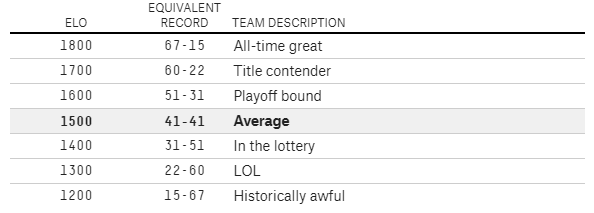
\includegraphics[width=.49\linewidth]{./EloChart} 

}

\caption{\label{fig:elo_chart}Breakdown of Elo Rating}\label{fig:unnamed-chunk-21}
\end{figure}

\begin{longtable}[]{@{}ll@{}}
\toprule
Statistics & Meaning\tabularnewline
\midrule
\endhead
G & Num. games played\tabularnewline
MP & Num. minutes played\tabularnewline
PER & Measure of per-minute production\tabularnewline
TS. & Overall shooting efficiency\tabularnewline
X3PAr & \% of field goal attempts from 3-point range\tabularnewline
FTr & Num. free throw attempts per field goal attempt\tabularnewline
ORB. & \% of available offensive rebounds that a player
grabbed\tabularnewline
DRB. & \% of available defensive rebounds that a player
grabbed\tabularnewline
TRB. & \% of available total rebounds that a player
grabbed\tabularnewline
AST. & \% of teammate field goals that a player assisted\tabularnewline
STL. & \% of opponent possessions that were stolen by a
player\tabularnewline
BLK. & \% of opponent field goals attempts that were blocked by a
player\tabularnewline
TOV. & Num. turnovers committed per 100 plays\tabularnewline
USG. & \% of team plays used by a player\tabularnewline
OWS & Num. wins contributed by a player from his offense\tabularnewline
DWS & Num. wins contributed by a player from his defense\tabularnewline
WS & Num. wins contributed by a player\tabularnewline
WS.48 & Num. wins contributed by a player per 48 minutes\tabularnewline
OBPM & Offensive points per 100 possessions above a league-average
player\tabularnewline
DBPM & Defensive points per 100 possessions above a league-average
player\tabularnewline
BPM & Total points per 100 possessions above a league-average
player\tabularnewline
VORP & Points per 100 team possessions contributed by a player above a
replacement-level player\tabularnewline
\bottomrule
\end{longtable}

\hypertarget{references}{%
\section{References}\label{references}}

\begin{quote}
{[}1{]} List of all sporting events canceled around the world during the
coronavirus pandemic
(\url{https://www.espn.com/olympics/story/_/id/28824781/list-sporting-events-canceled-coronavirus})
\end{quote}

\begin{quote}
{[}2{]} Elo ratings system
(\url{https://en.wikipedia.org/wiki/Elo_rating_system})
\end{quote}

\begin{quote}
{[}3{]} FiveThirtyEight NBA Elo Ratings
(\url{https://fivethirtyeight.com/features/how-we-calculate-nba-elo-ratings/})
\end{quote}

\begin{quote}
{[}4{]} Compilation of in-depth NBA statistics
(\url{https://www.basketball-reference.com/})
\end{quote}

\begin{quote}
{[}5{]} Elo Ratings for NBA Teams
(\url{http://practicallypredictable.com/2018/04/15/elo-ratings-for-nba-teams/\#more-1019})
\end{quote}

\end{document}
